\documentclass{article}

\usepackage{tikz}
\usepackage[left = 2cm, right = 2cm, top = 2cm, bottom = 2cm]{geometry}
\usetikzlibrary{calc, shapes.multipart, chains, arrows}

\begin{document}

% Explication du principe d'un tableau cumulatif grâce à la géométrie

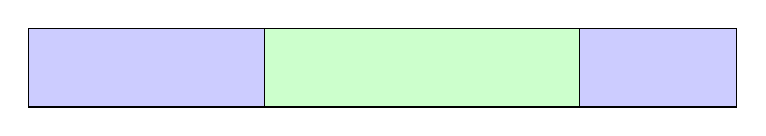
\begin{tikzpicture}
   \fill[blue!20, draw = black] (-2,0) rectangle (7,1);
   \fill[green!20, draw = black] (1,0) rectangle (5,1);
\end{tikzpicture}

\vspace{2cm}


\begin{tikzpicture}
   \fill[white] (-2,0) rectangle (7,1);
   \fill[green!20, draw = black] (1,0) rectangle (5,1);
   \node at (3,-0.5) {$=$};
\end{tikzpicture}

\vspace{0.25cm}

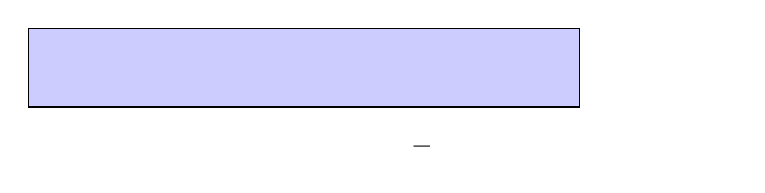
\begin{tikzpicture}
   \fill[white] (-2,0) rectangle (7,1);
   \fill[blue!20, draw = black] (-2,0) rectangle (5,1);
   \node at (3,-0.5) {$-$};
\end{tikzpicture}

\vspace{0.25cm}


\begin{tikzpicture}
   \fill[white] (-2,0) rectangle (7,1);
   \fill[blue!20, draw = black] (-2,0) rectangle (1,1);
\end{tikzpicture}

% Représentation des intervalles nécessaires

\newpage

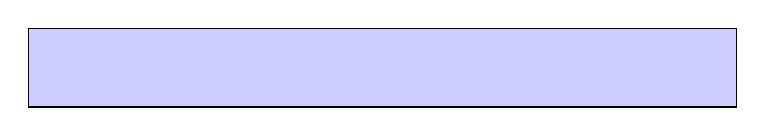
\begin{tikzpicture}
   \fill[blue!20, draw = black] (-2,0) rectangle (7,1);
\end{tikzpicture}

\vspace{1cm}
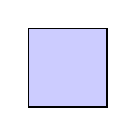
\begin{tikzpicture}
   \fill[blue!20, draw = black] (-2,0) rectangle (-1,1);
\end{tikzpicture}

\vspace{0.25cm}
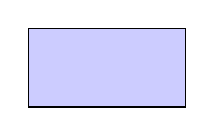
\begin{tikzpicture}
   \fill[blue!20, draw = black] (-2,0) rectangle (0,1);
\end{tikzpicture}

\vspace{0.25cm}
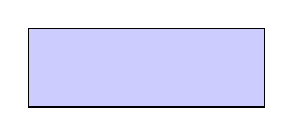
\begin{tikzpicture}
   \fill[blue!20, draw = black] (-2,0) rectangle (1,1);
\end{tikzpicture}

\vspace{0.25cm}
\begin{tikzpicture}
   \node (2,1) {$...$};
\end{tikzpicture}

\vspace{0.25cm}
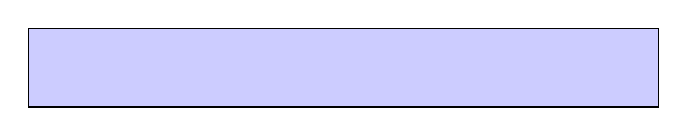
\begin{tikzpicture}
   \fill[blue!20, draw = black] (-2,0) rectangle (6,1);
\end{tikzpicture}

\vspace{0.25cm}
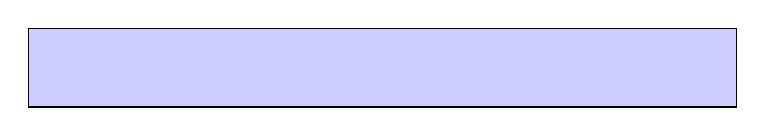
\begin{tikzpicture}
   \fill[blue!20, draw = black] (-2,0) rectangle (7,1);
\end{tikzpicture}

% Tableau cumulatif 2D : requête

\newpage

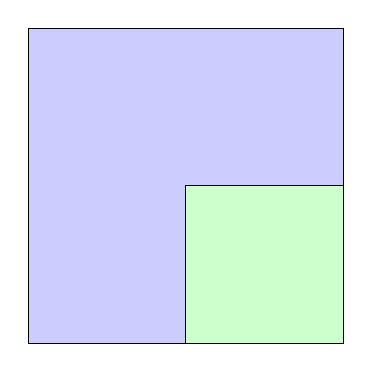
\begin{tikzpicture}
   \fill[blue!20, draw = black] (0,0) rectangle (4,4);
   \fill[green!20, draw = black] (2,0) rectangle (4,2);
\end{tikzpicture}

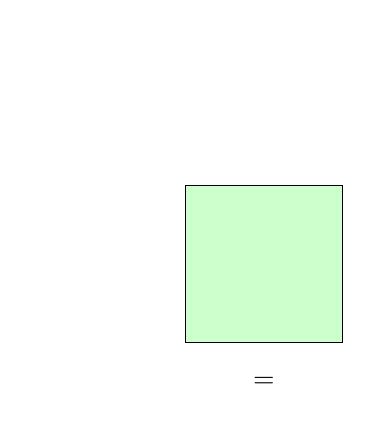
\begin{tikzpicture}
   \fill[white] (0,0) rectangle (4,4);
   \fill[green!20, draw = black] (2,0) rectangle (4,2);
   \node at (3,-0.5) {$=$};
\end{tikzpicture}

\vspace{0.25cm}

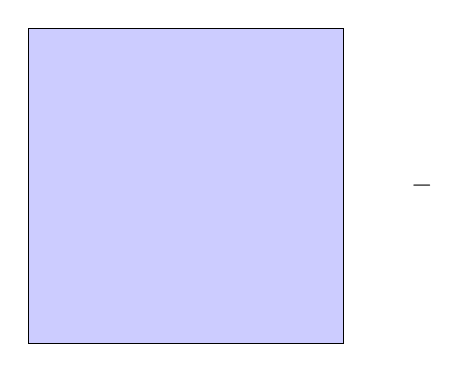
\begin{tikzpicture}
   \fill[blue!20, draw = black] (0,0) rectangle (4,4);
   \node at (5,2) {$-$};
\end{tikzpicture}
\hspace{0.25cm}
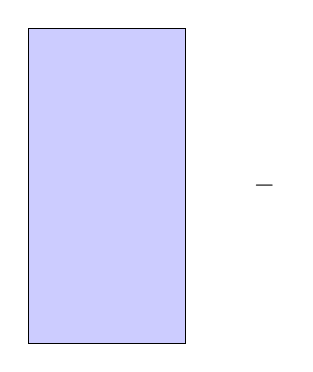
\begin{tikzpicture}
   \fill[blue!20, draw = black] (0,0) rectangle (2,4);
   \node at (3,2) {$-$};
\end{tikzpicture}
\hspace{0.25cm}
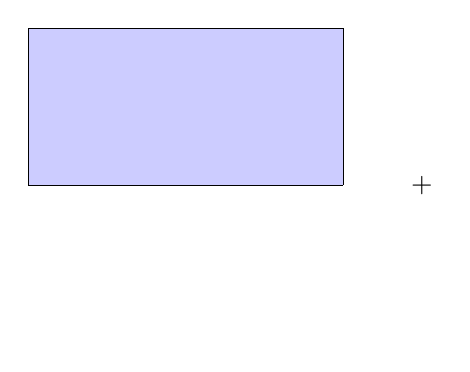
\begin{tikzpicture}
   \fill[blue!20, draw = black] (0,0) rectangle (4,4);
   \fill[white, draw = white] (0,0) rectangle (4,2);
   \draw (0,2) -- (4,2);
   \node at (5,2) {$+$};
\end{tikzpicture}
\hspace{0.25cm}
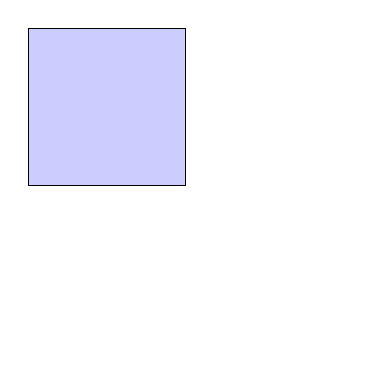
\begin{tikzpicture}
   \fill[blue!20, draw = black] (0,0) rectangle (2,4);
   \fill[white, draw = white] (0,0) rectangle (4,2);
   \draw (0,2) -- (2,2);
\end{tikzpicture}

% Tableau cumulatif 2D : initialisation

\newpage

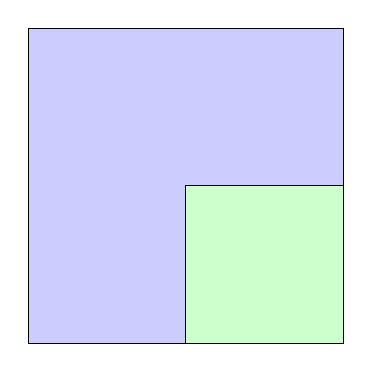
\begin{tikzpicture}
   \fill[blue!20, draw = black] (0,0) rectangle (4,4);
   \fill[green!20, draw = black] (2,0) rectangle (4,2);
\end{tikzpicture}

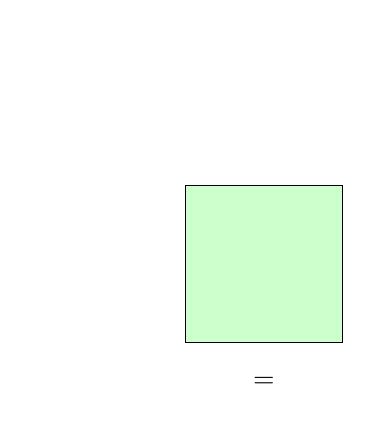
\begin{tikzpicture}
   \fill[white] (0,0) rectangle (4,4);
   \fill[green!20, draw = black] (2,0) rectangle (4,2);
   \node at (3,-0.5) {$=$};
\end{tikzpicture}

\vspace{0.25cm}

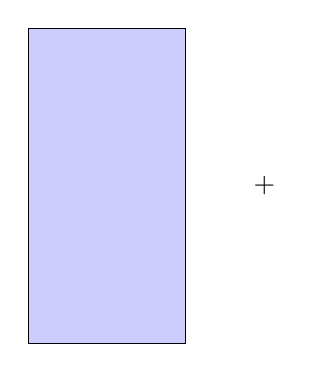
\begin{tikzpicture}
   \fill[blue!20, draw = black] (0,0) rectangle (2,4);
   \node at (3,2) {$+$};
\end{tikzpicture}
\hspace{0.25cm}
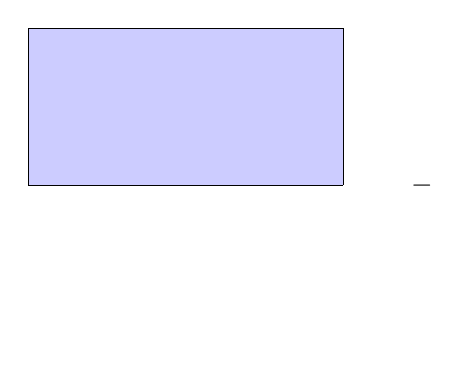
\begin{tikzpicture}
   \fill[blue!20, draw = black] (0,0) rectangle (4,4);
   \fill[white, draw = white] (0,0) rectangle (4,2);
   \draw (0,2) -- (4,2);
   \node at (5,2) {$-$};
\end{tikzpicture}
\hspace{0.25cm}
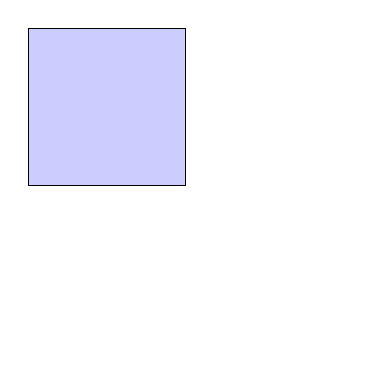
\begin{tikzpicture}
   \fill[blue!20, draw = black] (0,0) rectangle (2,4);
   \fill[white, draw = white] (0,0) rectangle (4,2);
   \draw (0,2) -- (2,2);
\end{tikzpicture}

\end{document}
